\chapter{Progettazione e implementazione}
\label{cap:progettazione-implementazione}

\intro{In questo capitolo, vengono descritte le scelte progettuali e le tecniche implementative utilizzate per realizzare il report delle vendite ed il sistema di raccomandazione. Si inizia con una panoramica del flusso delle attività, seguita da una descrizione delle tecnologie e degli strumenti utilizzati. Successivamente, si approfondiscono i vari componenti del sistema sviluppato.}

\section{Flusso delle attività}

\begin{figure}[!h]
    \centering 
    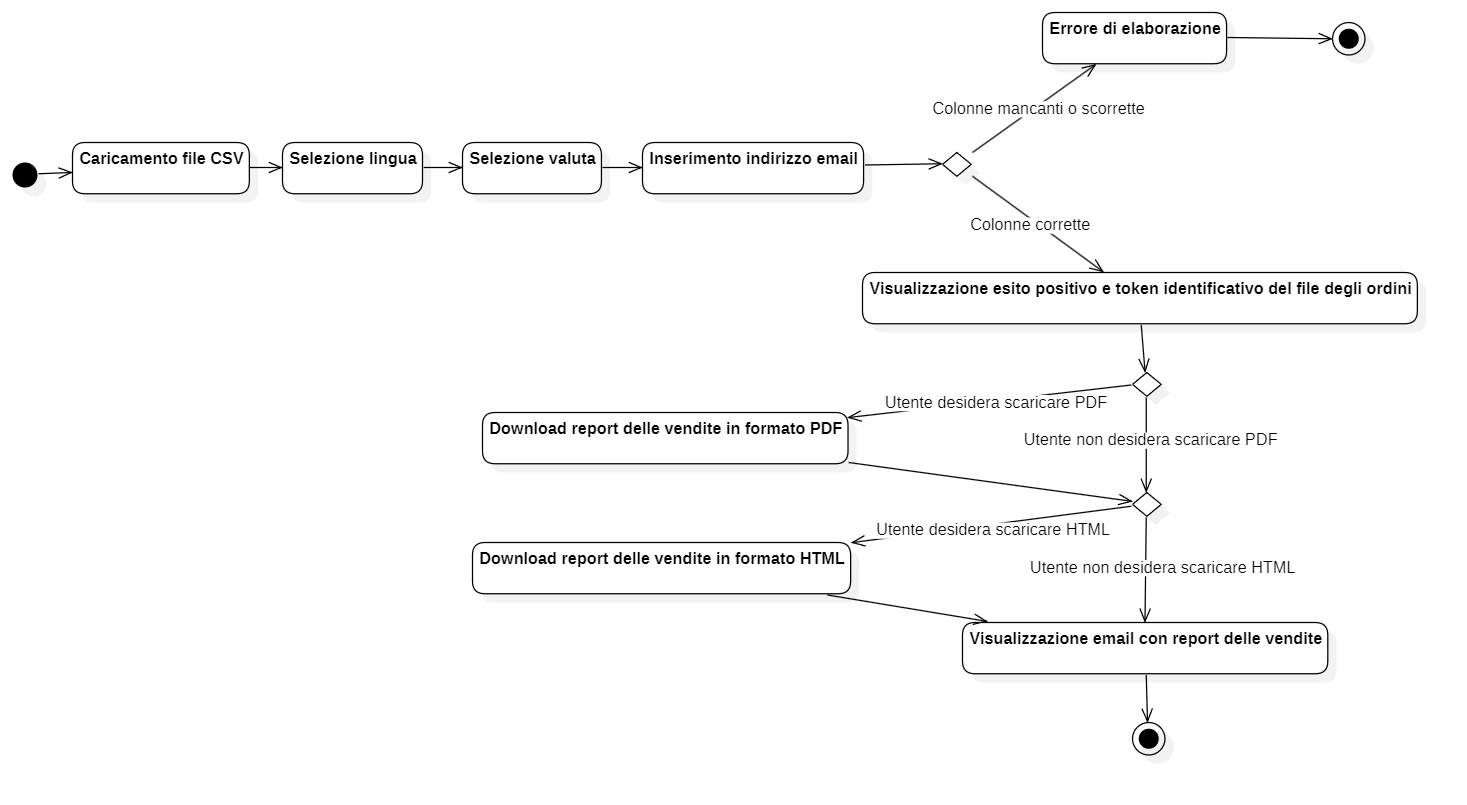
\includegraphics[width=0.9\columnwidth]{activity/Task di analisi delle vendite.png}
    \caption{Flusso delle attività della task di analisi delle vendite}
    \label{fig:activity-sales-analysis}
\end{figure}

Il flusso delle attività per la task di analisi delle vendite è rappresentato nella figura \ref{fig:activity-sales-analysis}. Le attività in sequenza previste dalla task dal lato dell'utente sono:
\begin{itemize}
    \item \textbf{Compilazione dei campi di input}: l'utente deve compilare i campi di input richiesti, cioè deve selezionare il file CSV contenente i dati delle vendite, selezionare la lingua del report e la valuta da utilizzare per i prezzi, e inserire l'indirizzo email a cui inviare il report;
    \item \textbf{Possibili output}: nel caso in cui l'utente abbia inserito correttamente i campi di input e nel caso la task non abbia riscontrato errori, l'utente visualizzerà un messaggio di esito positivo ed un invito a controllare la propria email per il report generato. Viene inoltre segnalata la generazione delle matrici di raccomandazione, e viene visualizzato il token che serve copiare per poter usufruire della task di raccomandazione. In caso la task non vada a buon fine, l'utente visualizzerà un messaggio di errore;
    \item \textbf{I file generati}: la task genera un file PDF ed un file HTML contenenti il report delle vendite, e l'utente ha la possibilità di scaricarli dall'apposita schermata del portale Oribea;
    \item \textbf{La ricezione della mail}: l'utente riceve una mail all'indirizzo email inserito in precedenza, il cui body contiene l'HTML del report, e riporta come allegati il report delle vendite in formato PDF ed HTML; inoltre, viene mostrato anche qui il token che serve copiare per poter usufruire della task di raccomandazione.
\end{itemize}

\begin{figure}[!h]
    \centering 
    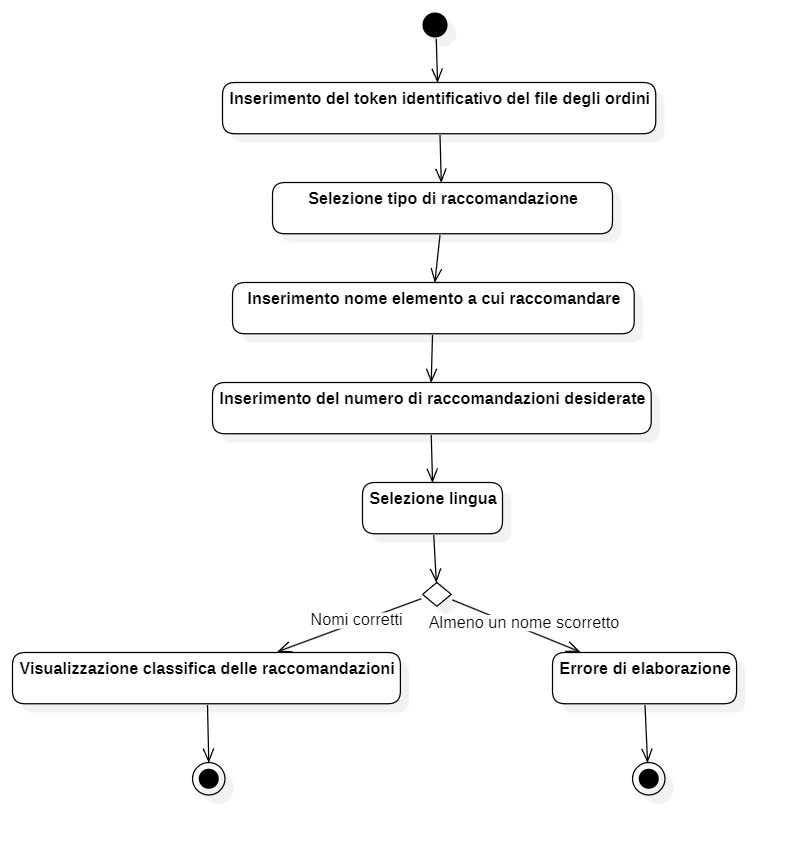
\includegraphics[width=0.9\columnwidth]{activity/Task di raccomandazione di prodotti e clienti.png}
    \caption{Flusso delle attività della task di raccomandazione di prodotti e clienti}
    \label{fig:activity-recommendation-products-customers}
\end{figure}

Il flusso delle attività per la task di raccomandazione di prodotti e clienti è rappresentato nella figura \ref{fig:activity-recommendation-products-customers}. Le attività in sequenza previste dalla task dal lato dell'utente sono:
\begin{itemize}
    \item \textbf{Compilazione dei campi di input}: l'utente deve compilare i campi di input richiesti, cioè deve inserire il token ricevuto nella mail della task di analisi delle vendite, selezionare il tipo di raccomandazione tra "Raccomandare prodotti per un cliente" e "Raccomandare clienti per un prodotto", inserire il nome dell'elemento a cui raccomandare, inserire il numero di raccomandazioni desiderate, e selezionare la lingua con cui presentare la classifica di raccomandazioni;
    \item \textbf{Possibili output}: nel caso in cui l'utente abbia inserito correttamente i campi di input e nel caso la task non abbia riscontrato errori, l'utente visualizzerà la classifica di raccomandazioni generata. In caso la task non vada a buon fine, l'utente visualizzerà un messaggio di errore.
\end{itemize}


\section{Tecnologie e strumenti}
\label{sec:tecnologie-strumenti}

Di seguito viene data una panoramica delle tecnologie e strumenti utilizzati.

\subsection{Tecnologia 1}
Descrizione Tecnologia 1.

\subsection{Tecnologia 2}
Descrizione Tecnologia 2


\section{Architettura del sistema}



\section{Preprocessing}
\label{sec:preprocessing}

\subsection{Riconoscimento delle marche}
\label{sec:recognition-brands}

Per poter analizzare le vendite in modo più dettagliato, è stato pensato di introdurre una colonna "Marca" nei dataset, che potesse contenere il nome della marca del prodotto presente in tale riga. Per ottenere ciò, era dunque necessario sviluppare un sistema di riconoscimento delle marche. Sono state provate le seguenti strategie:
\begin{itemize}
    \item \textbf{Riconoscimento tramite dizionario}: è stato creato un dizionario contenente le marche più comuni, ma si è rivelato poco efficace, poiché molte marche non erano presenti nel dizionario e il riconoscimento era limitato;
    \item \textbf{Riconoscimento tramite regex}: è stato provato a utilizzare delle espressioni regolari per riconoscere le marche, ma si è rivelato poco efficace, poiché molte marche non seguivano uno schema comune e il riconoscimento era limitato;
    \item \textbf{Riconoscimento tramite modelli di \gls{ml}\glsfirstoccur{}}: è stato pensato di creare un modello di \gls{ml} per riconoscere le marche, ma si è rivelato poco efficace, poiché il dataset non era sufficientemente grande e vario per addestrare un modello affidabile, e soprattuto non erano disponibili le etichette necessarie per un addestramento supervisionato;
    \item \textbf{Riconoscimento tramite modelli di \gls{ner}\glsfirstoccur{}}: è stato provato ad utilizzare un modello di \gls{ner} sulle descrizioni dei prodotti e a selezionare le entità segnalate di tipo \emph{ORG} (organizzazione), ma si è rivelato poco efficace, poiché il modello non era stato addestrato specificamente per questo compito e il riconoscimento era limitato;
    \item \textbf{Riconoscimento tramite \gls{llm}\glsfirstoccur{}}: è stato provato ad utilizzare un modello di linguaggio di grandi dimensioni (\gls{llm}) per riconoscere le marche, e si è rivelato mediamente efficace, ma il riconoscimento di ciascuna marca richiedeva troppo tempo e tantissime chiamate \gls{api}\glsfirstoccur{}; allora, è stato fatto un tentativo di raggruppamento di più descrizioni da inviare assieme per il riconoscimento di più marche contemporaneamente, ma si è rivelato poco efficace, poiché il modello ogni tanto si dimenticava di alcune marche o ne aggiungeva qualcuna in più, totalmente senza motivo (avvenivano cioè le cosidette "allucinazioni").
\end{itemize}

Dunque, si è deciso di non implementare il riconoscimento delle marche nel sistema di analisi automatizzato, poiché non era possibile garantire un riconoscimento affidabile e preciso.


\subsection{Riconoscimento delle categorie}
\label{sec:recognition-categories}

Per poter analizzare le vendite in modo più dettagliato, è stato pensato di introdurre una colonna "Categoria" nei dataset, che potesse contenere il nome della categoria del prodotto presente in tale riga. Per ottenere ciò, era dunque necessario sviluppare un sistema di riconoscimento delle categorie.

Escluse le opzioni già descritte nella sezione \ref{sec:recognition-brands} per il riconoscimento delle marche, è stato pensato di utilizzare un modello \gls{kmeans}\glsfirstoccur{} per raggruppare i prodotti in base alle loro descrizioni, in modo da ottenere delle categorie. Tuttavia, ciò si è rivelato poco efficace, poiché il modello non era in grado di raggruppare i prodotti in categorie in modo affidabile e preciso, e il numero di categorie era troppo elevato per poterle gestire manualmente.

Dunque, si è deciso di non implementare il riconoscimento delle categorie nel sistema di analisi automatizzato, poiché non era possibile garantire un riconoscimento affidabile e preciso.\\



\section{Language processing}
\label{sec:language-processing}

\section{Report}
\subsection{PDF}
\subsection{HTML}

\section{Invio di email}

\section{Le matrici di raccomandazione}
\subsection{Formato di archiviazione delle matrici}

\section{La predizione e rank fusion}

\section{Valutazione delle raccomandazioni}

\section{Collegamento con Google Cloud}
\subsection{Google Cloud Storage}
\subsection{Google Cloud Functions}
